\chapter{Results \& Discussion} \label{ch:results}

This chapter presents the quantitative results of the developed EPEC modeling framework. To comprehensively evaluate the impact of multi-service market participation on the strategic allocation of BESS, a comparative analysis is conducted between two distinct market setups: an \textbf{Energy-Only Scenario} (focused solely on day-ahead spot market arbitrage) and a \textbf{Multi-Service Scenario} (co-optimizing spot arbitrage with continuous aFRR provision). 

The Energy-Only setup serves as a benchmark, reflecting the focus of conventional BESS allocation models. By explicitly contrasting it with the Multi-Service setup, this comparison aims to isolate and quantify the specific effects of reserve market obligations on strategic investment decisions. The objective of this comparison is to demonstrate how lucrative capacity premiums and the resulting power bottlenecks fundamentally alter optimal BESS sizing.

The remainder of this chapter is organized as follows. Following a brief evaluation of the algorithmic convergence and stability of the EPEC framework, Section \ref{sec:allocation} analyzes the strategic investment behavior regarding spatial distribution (siting), power capacity (MW), and the resulting Energy-to-Power (E/P) ratios. Section \ref{sec:revenue_breakdown} breaks down the distinct revenue streams and investigates the spillover effect of the aFRR market on the arbitrage market. Finally, the chapter evaluate the aggregated system balance and nodal price dynamics, illustrating how multi-service obligations synchronize BESS operations across structurally diverse network nodes.

\section{Algorithmic Performance and EPEC Stability}
As detailed in Section \ref{sect:EPEC_Solution_Strategy}, solving the EPEC relies on a parallelized Gauss-Jacobi diagonalization algorithm, with convergence achieved when the \textit{Max Delta} of the installed capacity falls below 0.5 MW. The practical execution of both scenarios demonstrates that the model tweaks introduced in Section \ref{subsect:Model_Tweaks} were strictly necessary to stabilize the framework. Figure \ref{fig:convergence} illustrates the convergence history for both the Energy-Only and the Multi-Service scenarios, tracking the \textit{Max Delta} metric of the installed capacity.

\begin{figure}[htbp]
     \centering
     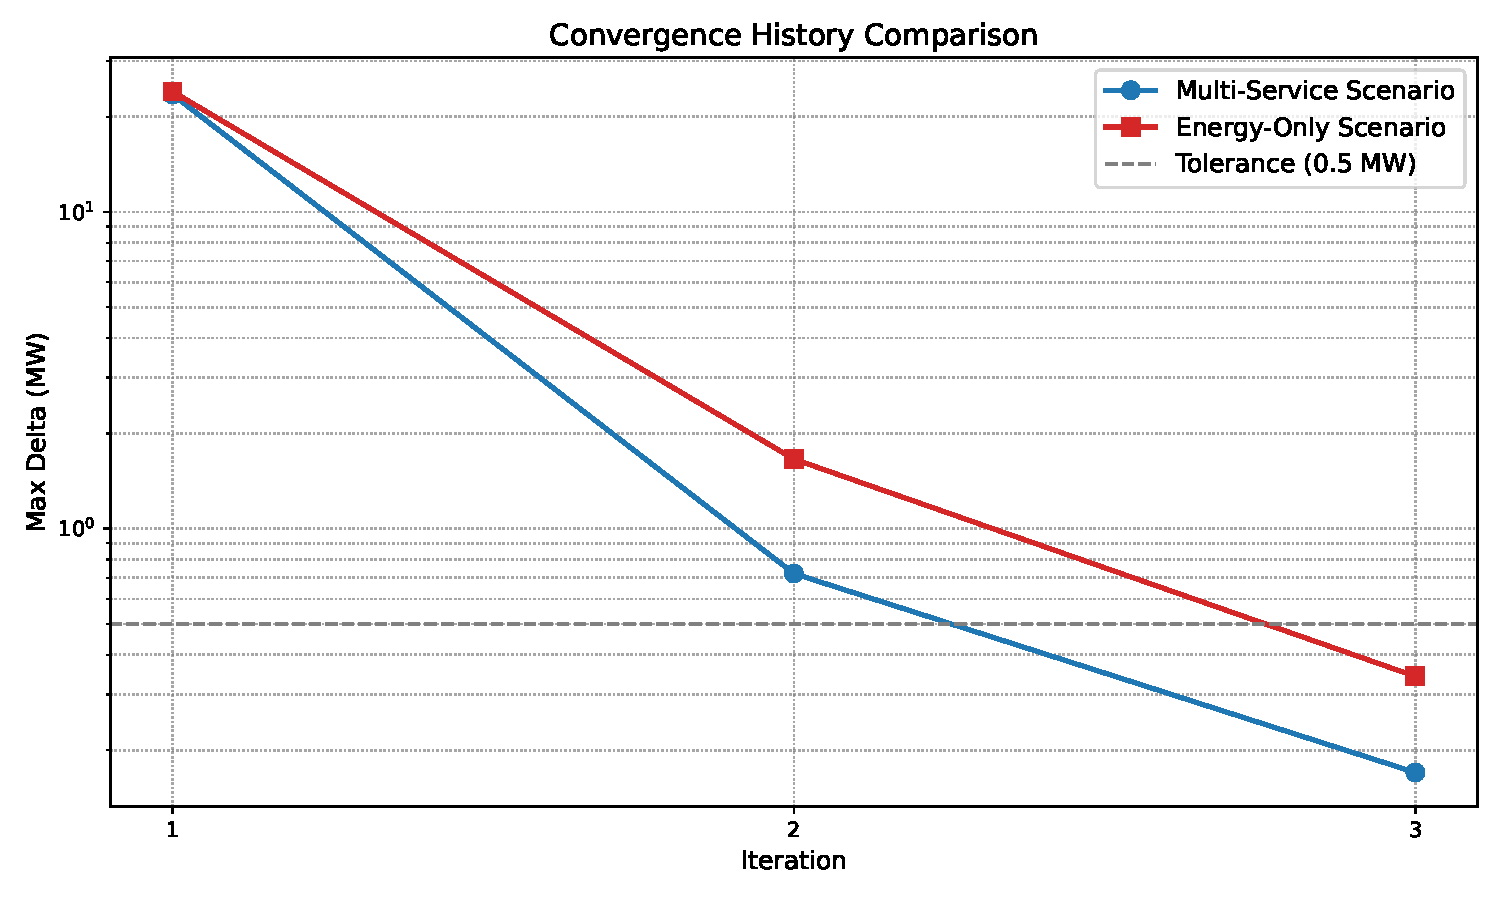
\includegraphics[width=\linewidth]{figures/Convergence_History_Comparison.pdf}
     \label{fig:convergence_without_afrr}
     \caption{Convergence history comparison displaying the \textit{Max Delta} in MW per iteration.}
     \label{fig:convergence}
\end{figure}

In contrast to typical EPEC behaviors documented in the literature, where pure arbitrage trading often leads to continuous "zig-zag" oscillations, the Energy-Only Scenario converged exceptionally fast. By optimizing strictly against the pre-calculated residual load of their rivals, the strategic investors accurately anticipated market price shifts. Combined with a damping factor of 0.25, the algorithm reliably reached a stable Nash Equilibrium in only 3 iterations, well below the strict tolerance threshold of 0.5 MW.
The Multi-Service Scenario exhibited identical, rapid convergence. Despite the additional mathematical stiffness introduced by the simultaneous co-optimization of strict state-of-charge constraints for aFRR blocks, the model terminated optimally after 3 iterations. The replacement of rigid KKT-deficit rules with the continuous Cournot pricing mechanism eliminated all previously observed exploits, seamlessly guiding the competitive oligopoly into a stable and mathematically sound equilibrium.

\section{Strategic BESS Allocation: Siting, Sizing, and the E/P Ratio} \label{sec:allocation}

The transition from a pure energy arbitrage market to a multi-service environment fundamentally alters the strategic investment behavior of the agents. By examining the results of the Energy-Only and Multi-Service scenarios, distinct patterns in spatial distribution (siting), power capacity (sizing in MW), and energy capacity (sizing in MWh) emerge.

In both scenarios, the total installed power capacity approaches the theoretical physical limits of the network. The shared connection limit of 100 MW per node is fully utilized across all five nodes, resulting in a total aggregated capacity that closely approaches the system-wide maximum of 500 MW. The perfectly balanced spatial distribution and the absence of any nodal overbooking demonstrate that the solver correctly and strictly enforces the hard boundaries of the shared resource constraints.

Furthermore, the continuous Cournot Inverse Demand curve establishes a highly competitive and balanced oligopoly. As detailed in Table \ref{tab:investment_stats}, the power capacity provision is shared almost equally among all participants in the Multi-Service scenario, with each investor installing approximately 124 MW. The varying discount rates (cost of capital ranging from 8\% to 20\%) do not lead to the exclusion of any participant from the power capacity market. Instead, the investors strategically share the capacity provision to maintain high endogenous clearing prices, deliberately avoiding the price collapse that would occur if a single investor oversupplied the reserve market.

While the nominal power capacity (MW) is evenly distributed among the competitors, the fundamental impact of the investors' heterogeneous risk affinity (represented by their individual discount rates) becomes highly evident in their energy capacity (MWh) sizing. As established in the methodology (Section \ref{subsect:BESS_Characteristics}), a minimum Energy-to-Power (E/P) ratio of 2.0 hours is enforced. However, the endogenously optimized configurations deviate significantly from this baseline, especially when multi-service requirements are introduced.

In the Multi-Service Scenario, the simultaneous co-optimization of 4-hour aFRR blocks and spot market arbitrage requires substantial energy reservoirs to compensate for the severe power bottleneck created by continuous reserve provision. Because the capacity is blocked for the highly profitable aFRR market, the batteries are stripped of their operational flexibility. Investor 1, possessing the lowest cost of capital ($r = 0.08$), leverages its financial advantage to install a massive energy capacity of 2,648.58 MWh, resulting in an exceptionally high E/P ratio of 21.21 hours. Overlooking the unrealistic project size, this "patient" investor can amortize the immense upfront CAPEX for cheap battery cells over the 15-year project lifetime to extract marginal revenues out of the spot market with its remaining fractional power capacity.

Conversely, investors with higher capital costs cannot afford such capital-intensive energy reservoirs. Investor 2 ($r = 0.12$), for instance, restricts its energy capacity to 291.13 MWh, resulting in an E/P ratio of 2.35 hours---staying very close to the technical minimum to minimize investment costs. This empirical finding highlights a crucial dynamic in liberalized multi-service storage markets: the cost of capital is the primary driver for the depth of storage (energy capacity) rather than the nominal power capacity (MW) in an oligopolistic setting.

\begin{table}[htpb]
    \centering
    \caption{Aggregated BESS investment metrics comparing the Energy-Only and Multi-Service scenarios.}
    \label{tab:investment_stats}
    \makebox[\textwidth][c]{
        \begin{tabular}{lc | ccc | ccc}
            \toprule
            & & \multicolumn{3}{c|}{\textbf{Energy-Only Scenario}} & \multicolumn{3}{c}{\textbf{Multi-Service Scenario}} \\
            \cmidrule{3-8}
            \textbf{Investor} & \textbf{WACC} & \textbf{Total MW} & \textbf{Total MWh} & \textbf{E/P Ratio} & \textbf{Total MW} & \textbf{Total MWh} & \textbf{E/P Ratio} \\
            \midrule
            Investor 1 & 8.0\%  & 122.22 & 484.32  & 3.96  & 124.90 & 2648.58 & 21.21 \\
            Investor 2 & 12.0\% & 126.57 & 2392.83 & 18.91 & 123.62 & 291.13  & 2.35  \\
            Investor 3 & 15.0\% & 124.42 & 758.93  & 6.10  & 123.99 & 716.09  & 5.78  \\
            Investor 4 & 20.0\% & 123.90 & 595.77  & 4.81  & 124.57 & 625.89  & 5.02  \\
            \bottomrule
        \end{tabular}
    }
\end{table}

\section{Revenue Stream Breakdown and the Arbitrage-Reserve Trade-off} \label{sec:revenue_breakdown}

The allocation of generation capacity is fundamentally driven by the expected profitability of the assets. Analyzing the revenue streams—specifically the distribution between day-ahead spot market arbitrage and aFRR capacity provision—reveals critical insights into the operational priorities forced upon the BESS by the market design. 

In the Energy-Only Scenario, the model demonstrates economically sound and rational arbitrage behavior. Given the calibrated system parameters (marginal generation costs of 40 €/MWh for base-load and 80 €/MWh for peak-load, alongside a degradation cost of 15 €/MWh), the price spreads are sufficient to offset efficiency losses and physical battery wear. As derived from the simulation logs, all four investors achieve solid, positive daily arbitrage profits ranging from approximately 52,600 € (Investors 3 and 4) to 68,200 € (Investor 2). The BESS assets act as pure price-takers in the time-shifting of energy, buying during low-price periods (high wind/PV feed-in) and discharging during peak residual load.

However, the introduction of the reserve market in the Multi-Service Scenario triggers a massive paradigm shift in revenue generation. Driven by the continuous Cournot Inverse Demand curve, the strategic investors form a highly profitable oligopoly in the aFRR market. By collectively withholding capacity to intentionally fulfill only a portion of the system operator's total reserve demand, the strategic actors keep the endogenous aFRR clearing price artificially high (near 600 €/MW per hour). Consequently, the primary source of income entirely shifts to the reserve market. As detailed in Table \ref{tab:revenue_stats}, daily aFRR revenues reach between 292,986 € and 293,041 € for Investors 2, 3, and 4. Investor 1, leveraging its massive energy capacity (E/P ratio of 21.21) and low capital costs, captures an even higher aFRR revenue of 332,852 €.

The overwhelming financial dominance of the reserve market comes at a severe operational cost, manifesting as stark arbitrage-reserve trade-off. While Investors 2, 3, and 4 see their spot market profits plummet to a fraction of their previous values (between 3,500 € and 4,500 €), Investor 1 deliberately operates its BESS at a spot market loss, generating a arbitrage loss of -2,574 € per day.

This counter-intuitive behavior is driven by a cross-market opportunity cost logic caused by a severe power bottleneck. Due to the high margins dictated by the Cournot inverse demand, investors strategically allocate almost their entire expensive inverter capacity (MW) to reserve provision. To still capture any remaining arbitrage spreads, investors drastically oversize their relatively cheap battery cell capacity (MWh), resulting in extraordinarily high Energy-to-Power (E/P) ratios (e.g., $> 21$ hours). The loss-making spot market operation is a direct consequence of this inverter capacity lock-up: the batteries are forced into highly inefficient, prolonged charge and discharge cycles just to squeeze marginal revenues out of the remaining fractional MW capacity, accepting operational spot market losses to sustain the overall profit-maximizing strategy.

Ultimately, the strategic investors willingly sacrifice spot market profitability, accepting negative arbitrage as an unavoidable opportunity cost necessary to unlock the vastly superior cartel profits of the aFRR oligopoly.

\begin{table}[htpb]
    \centering
    \caption{Daily revenue stream breakdown comparing Arbitrage and aFRR profits across the Energy-Only and Multi-Service scenarios.}
    \label{tab:revenue_stats}
    \makebox[\textwidth][c]{
        \begin{tabular}{lc | cc | cc}
            \toprule
            & & \multicolumn{2}{c|}{\textbf{Energy-Only Scenario}} & \multicolumn{2}{c}{\textbf{Multi-Service Scenario}} \\
            \cmidrule{3-6}
            \textbf{Investor} & \textbf{WACC} & \textbf{Arbitrage (€)} & \textbf{aFRR (€)} & \textbf{Arbitrage (€)} & \textbf{aFRR (€)} \\
            \midrule
            Investor 1 & 8.0\%  & 64,660.66 & 0.00 & -2,574.26 & 332,852.44 \\
            Investor 2 & 12.0\% & 68,297.04 & 0.00 & 4,521.00  & 292,986.68 \\
            Investor 3 & 15.0\% & 52,641.06 & 0.00 & 3,759.11  & 293,034.14 \\
            Investor 4 & 20.0\% & 52,686.17 & 0.00 & 3,532.13  & 293,041.04 \\
            \bottomrule
        \end{tabular}
    }
\end{table}

\section{System-Wide Operation Profiles and Grid Congestion} \label{sec:system_profiles}

Beyond financial revenue maximization, the strategic operation of the BESS portfolio has a profound physical impact on the power system. Analyzing the aggregated system balances (Figure \ref{fig:system_balance}) reveals how the BESS units dynamically adapt to renewable energy intermittency and diurnal demand patterns.

The temporal generation profiles in the test system create four distinct operational phases over the 24-hour period. During the night and early morning (hours 1 to 6), the system experiences high wind power feed-in coupled with low system demand. As observed in the system balance, the BESS portfolio aggressively charges during these hours (indicated by the negative net BESS power). This coordinated charging absorbs the excess renewable generation that would otherwise force the base-load generator to ramp down unnecessarily.

As the day progresses into the morning peak (hours 7 to 9), the system encounters its absolute daily maximum in load demand. Correspondingly, the BESS portfolio shifts into its primary discharging phase, reaching its maximum injection power for the day. This critical intervention supplies the high morning demand just before solar generation fully ramps up, actively preventing severe capacity shortages.

During the mid-day period (hours 10 to 15), the system is characterized by strong photovoltaic (PV) generation, significantly suppressing the residual load. The BESS units utilize this secondary low-price window to aggressively recharge and restore their state-of-charge. 

Conversely, during the evening peak (hours 17 to 21), when demand experiences a secondary surge and solar generation ceases, the BESS portfolio enters its second discharging phase. While the injection power is lower than during the morning peak, this operation remains vital. By injecting previously stored renewable energy into the grid, the storage units displace expensive peak-load generation, effectively capping the system-wide price spikes and supplying the evening demand.

While the fundamental time-shifting behavior is present in both scenarios, the Multi-Service Scenario introduces observable rigidities. In the Energy-Only setup, BESS operations perfectly mirror the spot price spreads, resulting in deep, continuous charge and discharge cycles. However, the requirement to provide continuous 4-hour reserve capacity blocks (aFRR) forces the BESS into shallower and more constrained spot market operations, as the batteries must maintain sufficient energy reservoirs for potential reserve activation.

These system-wide operations are intrinsically linked to the physical limitations of the transmission network. The accompanying line loading heatmaps (Figure \ref{fig:line_congestion}) illustrate the spatial grid utilization. Notably, transmission lines L14, L15, and L34 operate well below their thermal limits throughout the day. Instead of forcing power through constrained corridors, the previously discussed optimal sizing strategy (see Section \ref{sec:allocation})--where BESS capacity is evenly distributed across all five nodes--acts as a critical congestion relief mechanism. By charging locally during periods of excess generation and discharging locally during peak demand, the BESS portfolio effectively balances the system without pushing these transmission lines to their limits.

\begin{figure}[htbp]
    \centering
    \begin{subfigure}{0.48\linewidth}
        \centering
        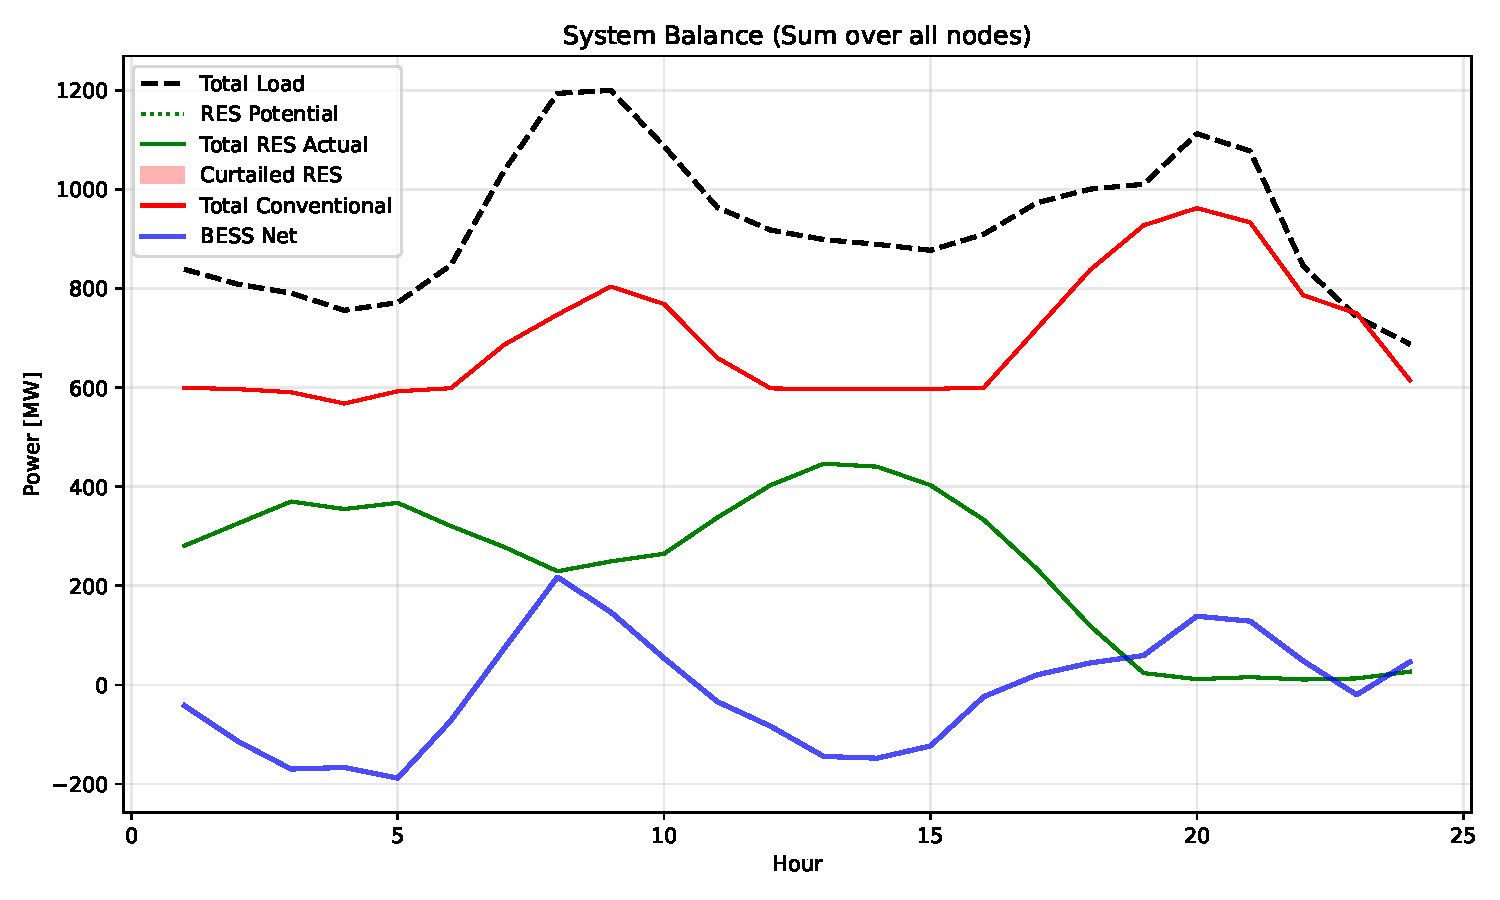
\includegraphics[width=\linewidth]{figures/without_aFRR_System_Balance.pdf}
        \caption{Energy-Only Scenario}
        \label{fig:balance_energy}
    \end{subfigure}
    \hfill
    \begin{subfigure}{0.48\linewidth}
        \centering
        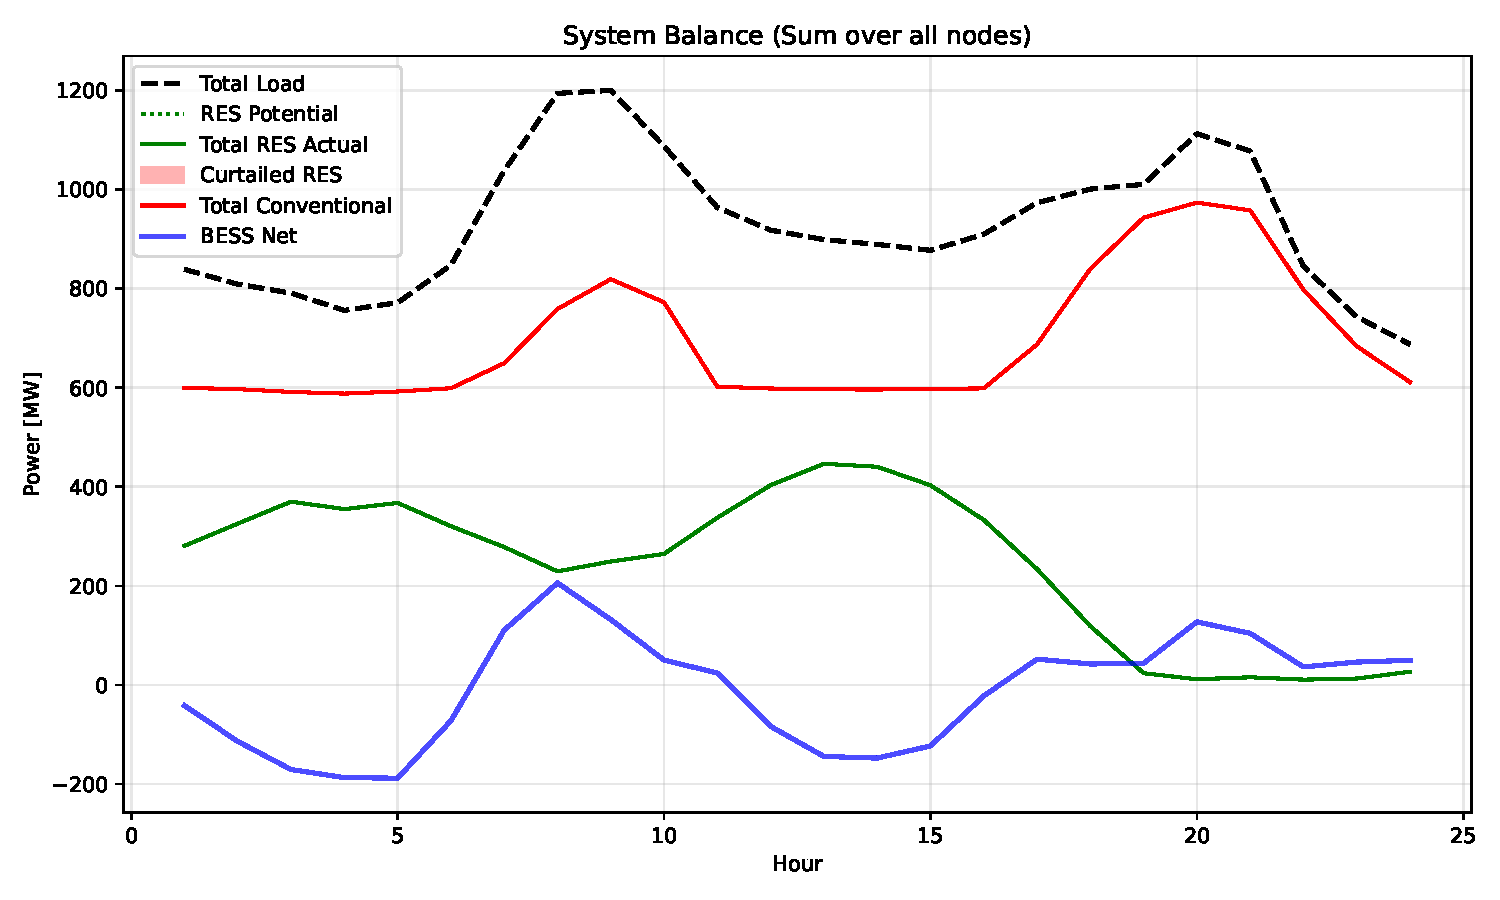
\includegraphics[width=\linewidth]{figures/with_aFRR_System_Balance.pdf}
        \caption{Multi-Service Scenario}
        \label{fig:balance_multi}
    \end{subfigure}
    \caption{Aggregated system balance over 24 hours. The solid blue line represents the net BESS dispatch (negative values indicate charging mode).}
    \label{fig:system_balance}
\end{figure}

\begin{figure}[htbp]
    \centering
    \begin{subfigure}{0.48\linewidth}
        \centering
        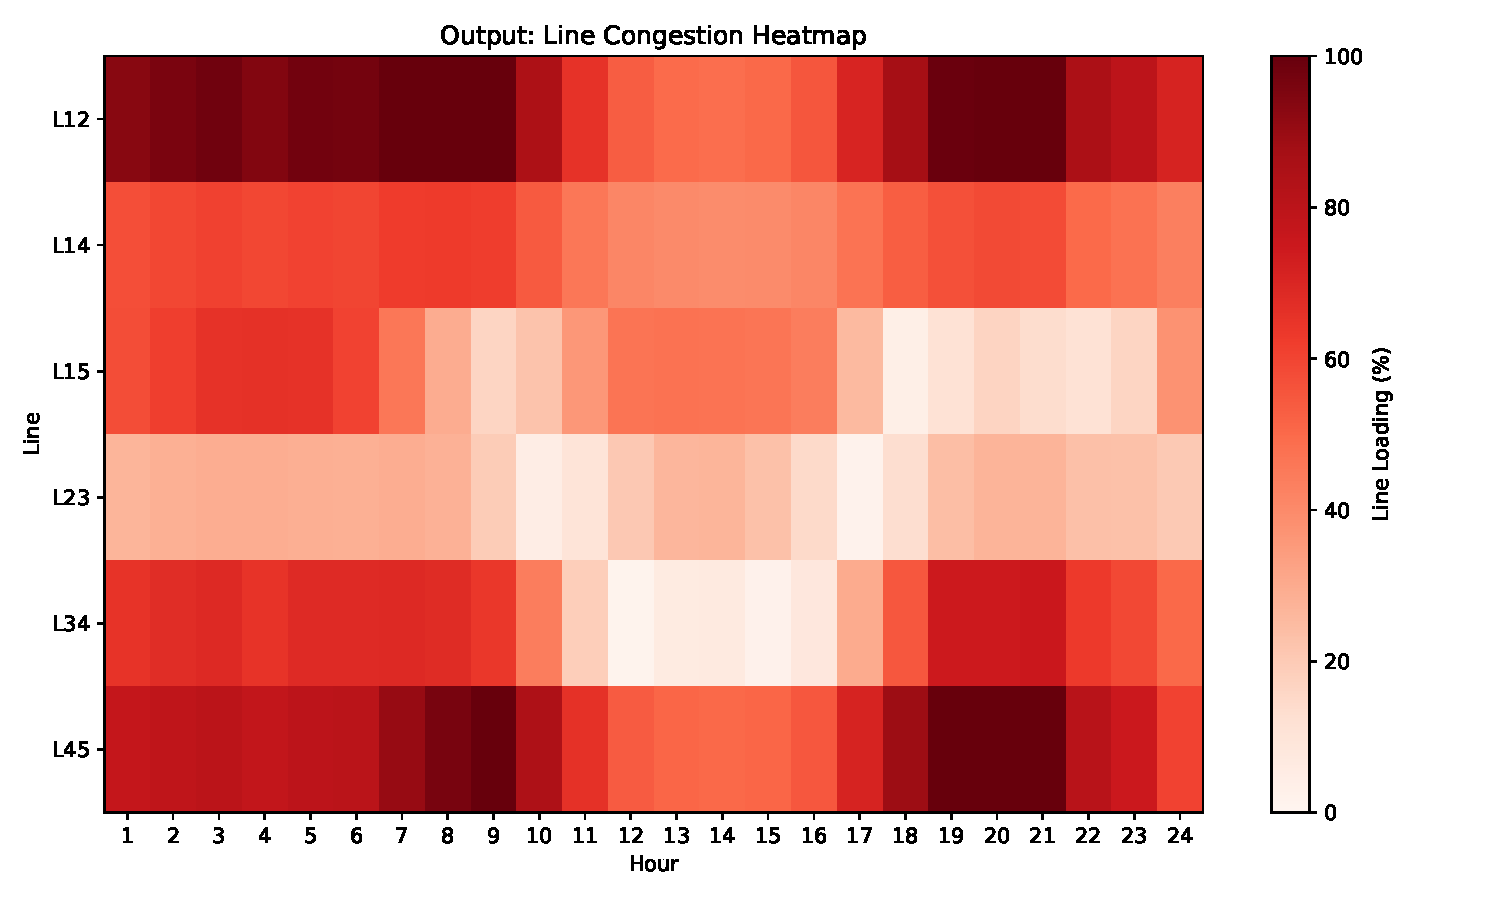
\includegraphics[width=\linewidth]{figures/without_aFRR_Line_Congestion.pdf}
        \caption{Energy-Only Scenario}
        \label{fig:congestion_energy}
    \end{subfigure}
    \hfill
    \begin{subfigure}{0.48\linewidth}
        \centering
        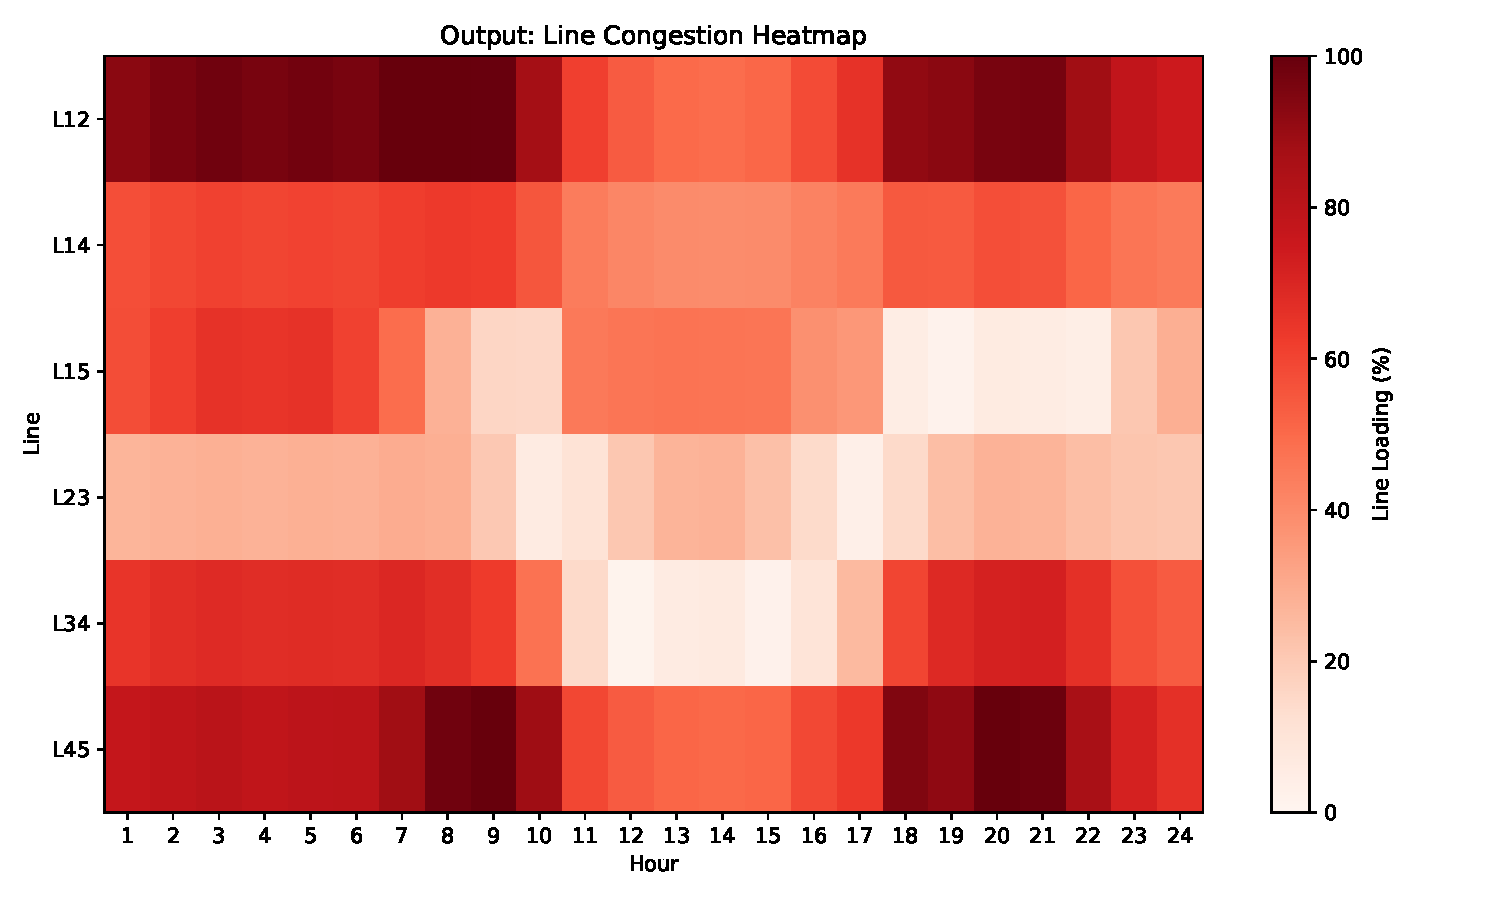
\includegraphics[width=\linewidth]{figures/with_aFRR_Line_Congestion.pdf}
        \caption{Multi-Service Scenario}
        \label{fig:congestion_multi}
    \end{subfigure}
    \caption{Heatmaps of transmission line loading. Lines L14, L15, L23 and L34 remain structurally unconstrained, demonstrating the effectiveness of locally distributed BESS capacities.}
    \label{fig:line_congestion}
\end{figure}

\section{Nodal Price Dynamics and Local Arbitrage} \label{sec:nodal_dynamics}

The aggregated system behavior discussed in the previous sections is fundamentally driven by the underlying Locational Marginal Prices (LMPs). In the decentralized MPEC framework, these nodal prices act as the primary scarcity signals, coordinating the competitive local arbitrage strategies of the BESS investors. Analyzing the individual nodal balances (Figures \ref{fig:n1_balance} and \ref{fig:n3_balance}) reveals extreme spatial price spreads generated by the heterogeneous distribution of generation assets and strict transmission limits.

In the Energy-Only Scenario, the price dynamics exhibit extreme local divergence. At Node 3 (PV-dominated), the LMP demonstrates severe scarcity pricing during the morning and evening system peaks, spiking from the 80 €/MWh peak-load marginal cost to over 600 €/MWh. The BESS portfolio logically reacts to these massive arbitrage opportunities by discharging heavily during these exact hours. 

Conversely, Node 1 (Wind and Base-Load) demonstrates a paradoxical price dynamic during the very same periods. While the rest of the system experiences peak demand and high prices, the local LMP at Node 1 drops from 80 €/MWh down to 40 €/MWh during the morning and evening peaks. This phenomenon is a textbook result of nodal pricing under structural grid congestion: the transmission line L12 hit their thermal limits, effectively isolating the node and trapping the cheap 40 €/MWh base-load generation locally. Despite these unexpectedly low local prices during peak hours, the BESS units still perform minor discharging operations, indicating complex interactions with their internal state-of-charge cycles.

While the Energy-Only setup highlights isolated local market conditions, the Multi-Service Scenario fundamentally disrupts this spatial divergence. The commitment to 4-hour aFRR blocks forces a systemic synchronization of BESS operations, which consequently homogenizes the nodal prices. 

This synchronization is clearly visible when comparing the operational strategies at Node 3 and Node 1. At Node 3, the morning price settles near 50 €/MWh, prompting the BESS to charge. The price then climbs to 80 €/MWh and holds until noon, triggering BESS discharge. As the mid-day PV peak hits, the price sharply drops to 40 €/MWh, creating a brief charging window, before surging back to 80 €/MWh at 16:00 due to high evening demand, leading to the final discharge phase. 

Remarkably, the price fluctuations and the BESS charging strategy at Node 1 mirror those at Node 3 almost identically. This demonstrates that the rigid state-of-charge requirements of the system-wide aFRR market completely dominate the operational logic of the batteries. The localized network constraints and nodal scarcity signals, which defined the Energy-Only scenario, are largely overridden by the lucrative, yet inflexible, obligations of the reserve market.

\begin{figure}[htbp]
    \centering
    \begin{subfigure}{0.75\linewidth}
        \centering
        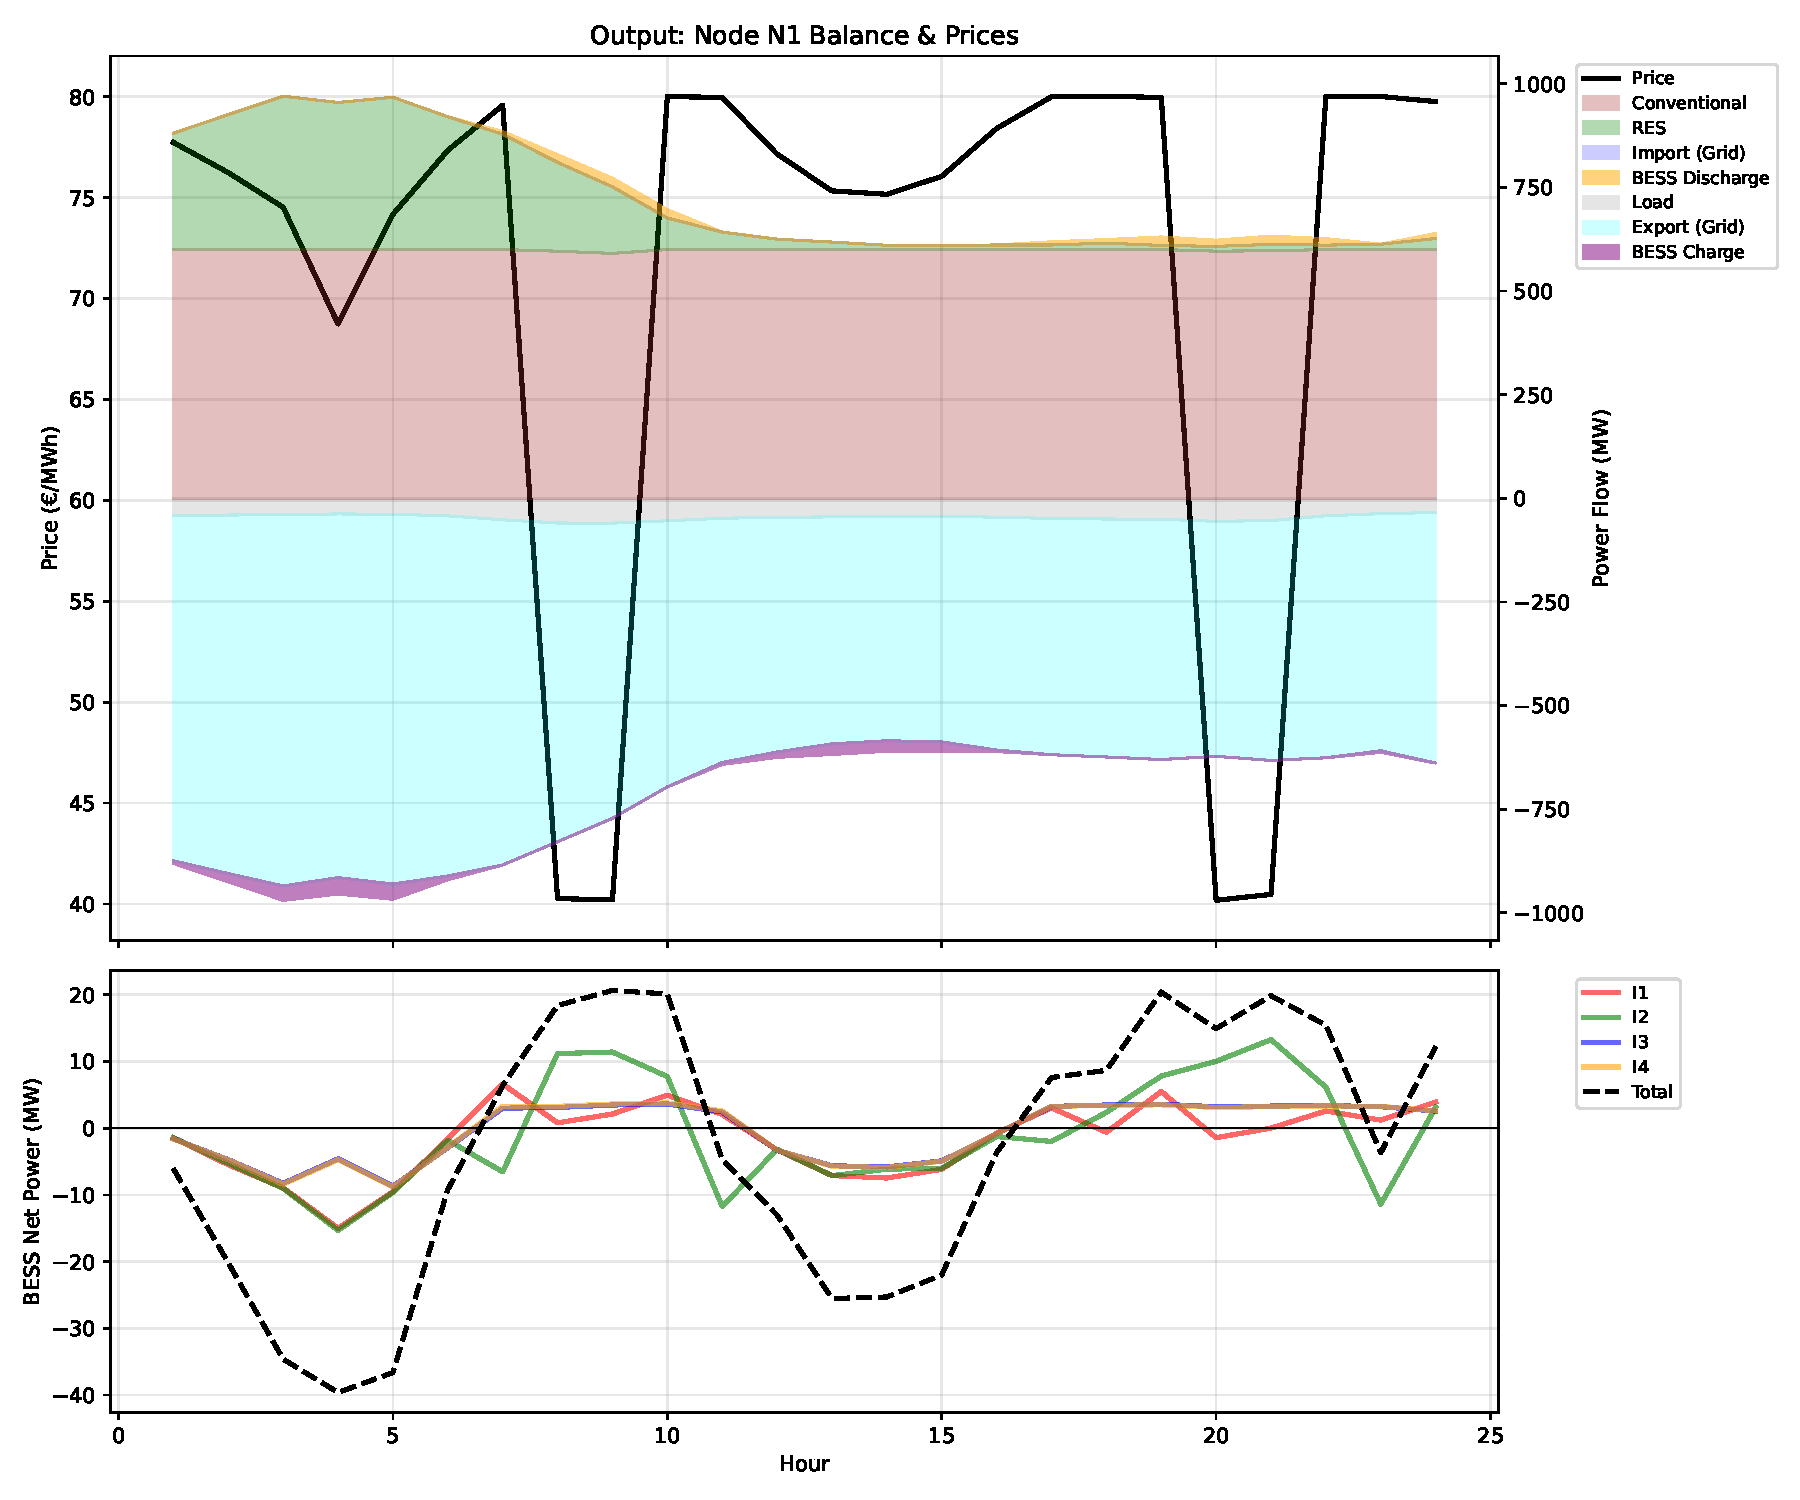
\includegraphics[width=\linewidth]{figures/without_aFRR_N1_Balance.pdf}
        \caption{Node 1 (Energy-Only)}
        \label{fig:n1_energy}
    \end{subfigure}
    \hfill
    \begin{subfigure}{0.75\linewidth}
        \centering
        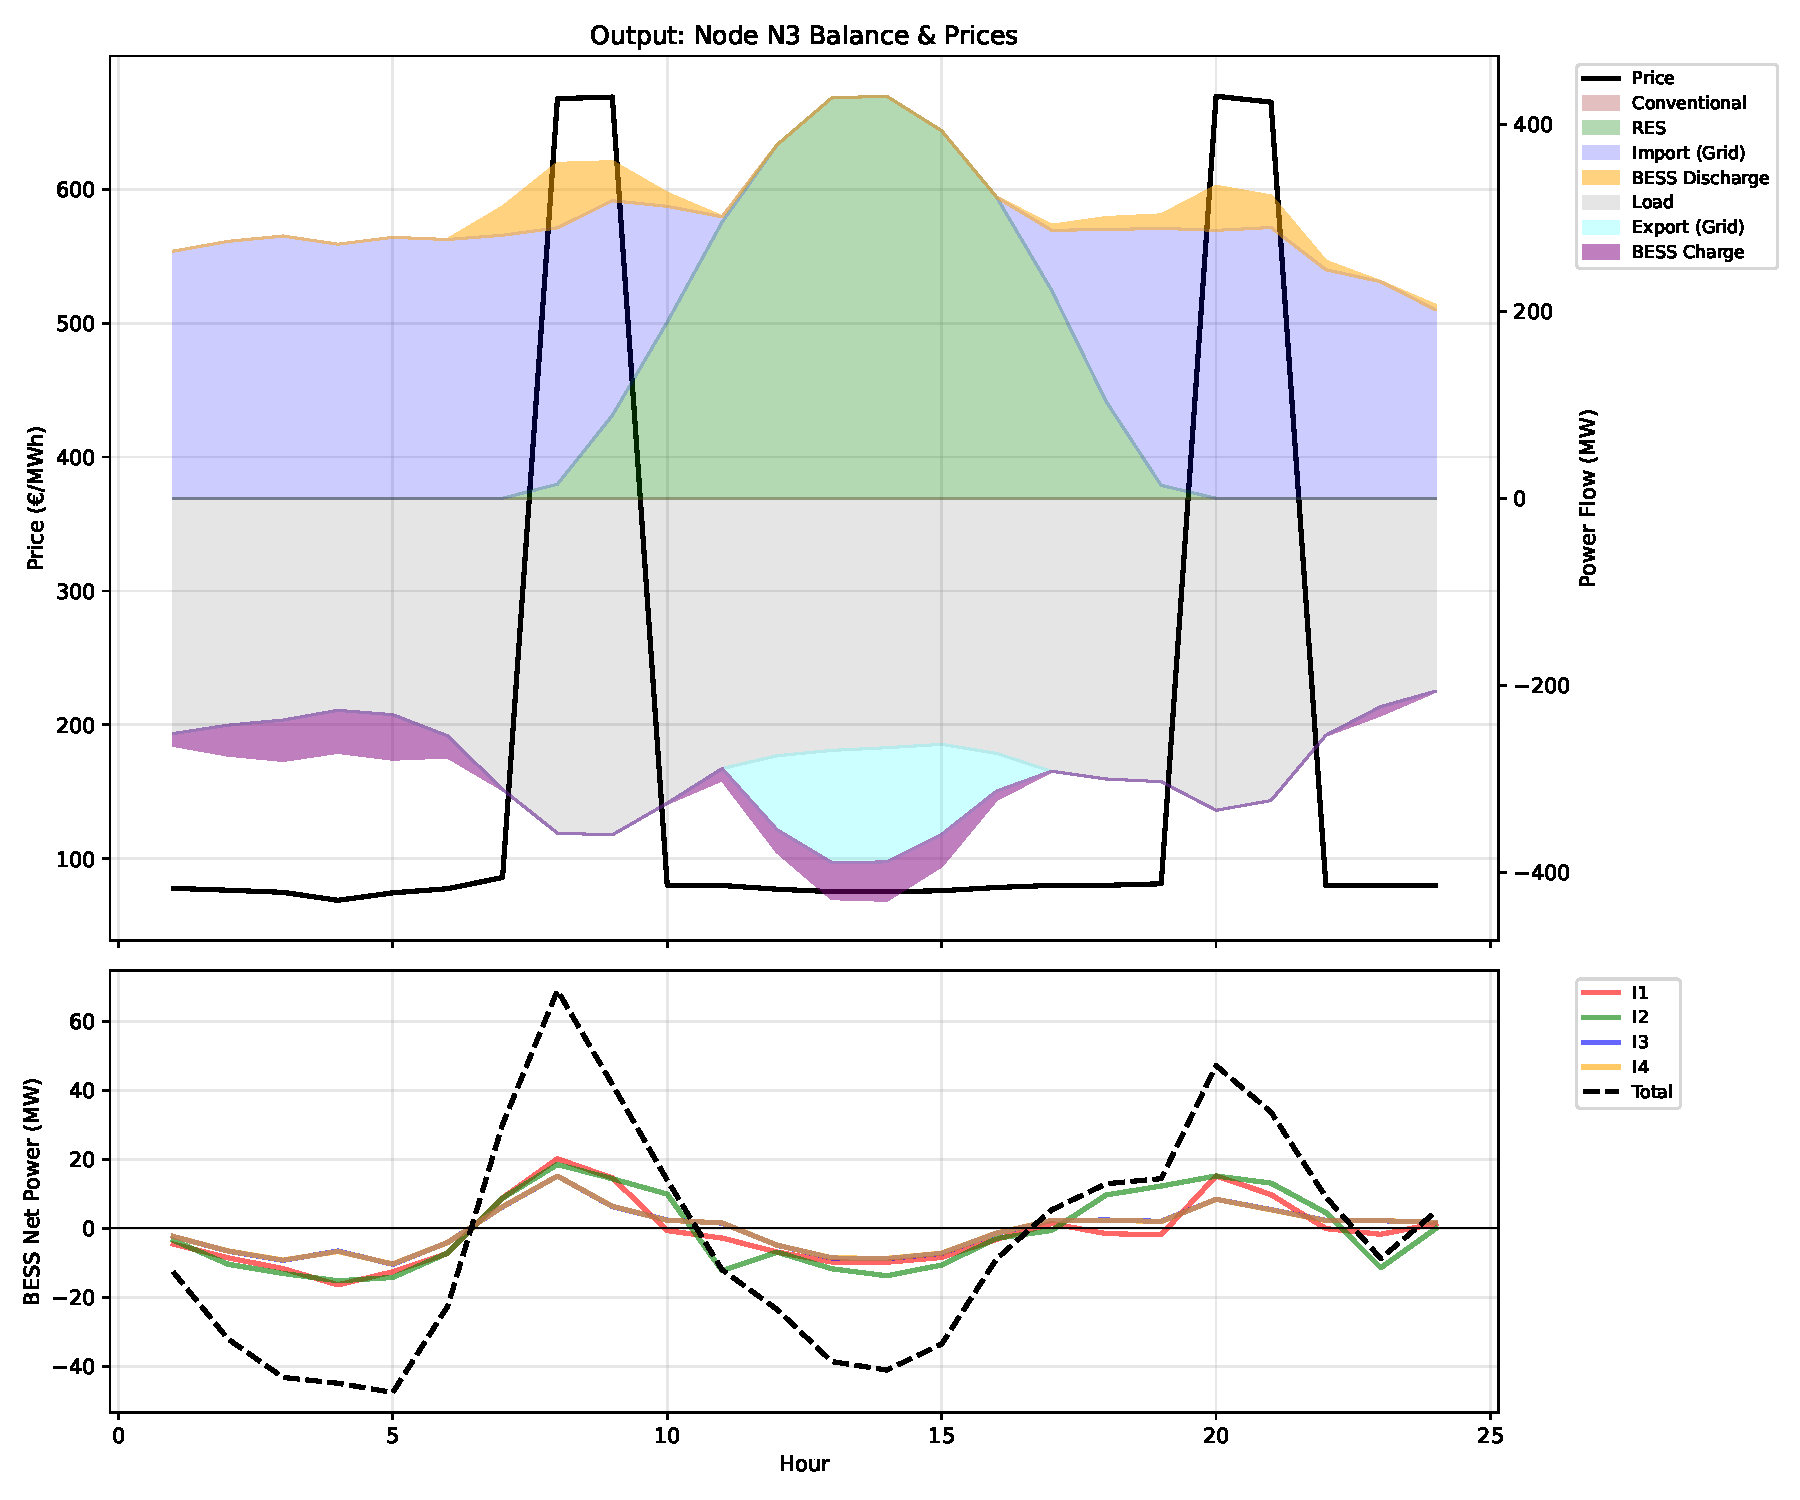
\includegraphics[width=\linewidth]{figures/without_aFRR_N3_Balance.pdf}
        \caption{Node 3 (Energy-Only)}
        \label{fig:n3_energy}
    \end{subfigure}
    \caption{Nodal balances in the Energy-Only Scenario. Notice the scarcity price spikes at N3 and the paradoxical price drops at N1 during system peaks.}
    \label{fig:n1_balance}
\end{figure}

\begin{figure}[htbp]
    \centering
    \begin{subfigure}{0.75\linewidth}
        \centering
        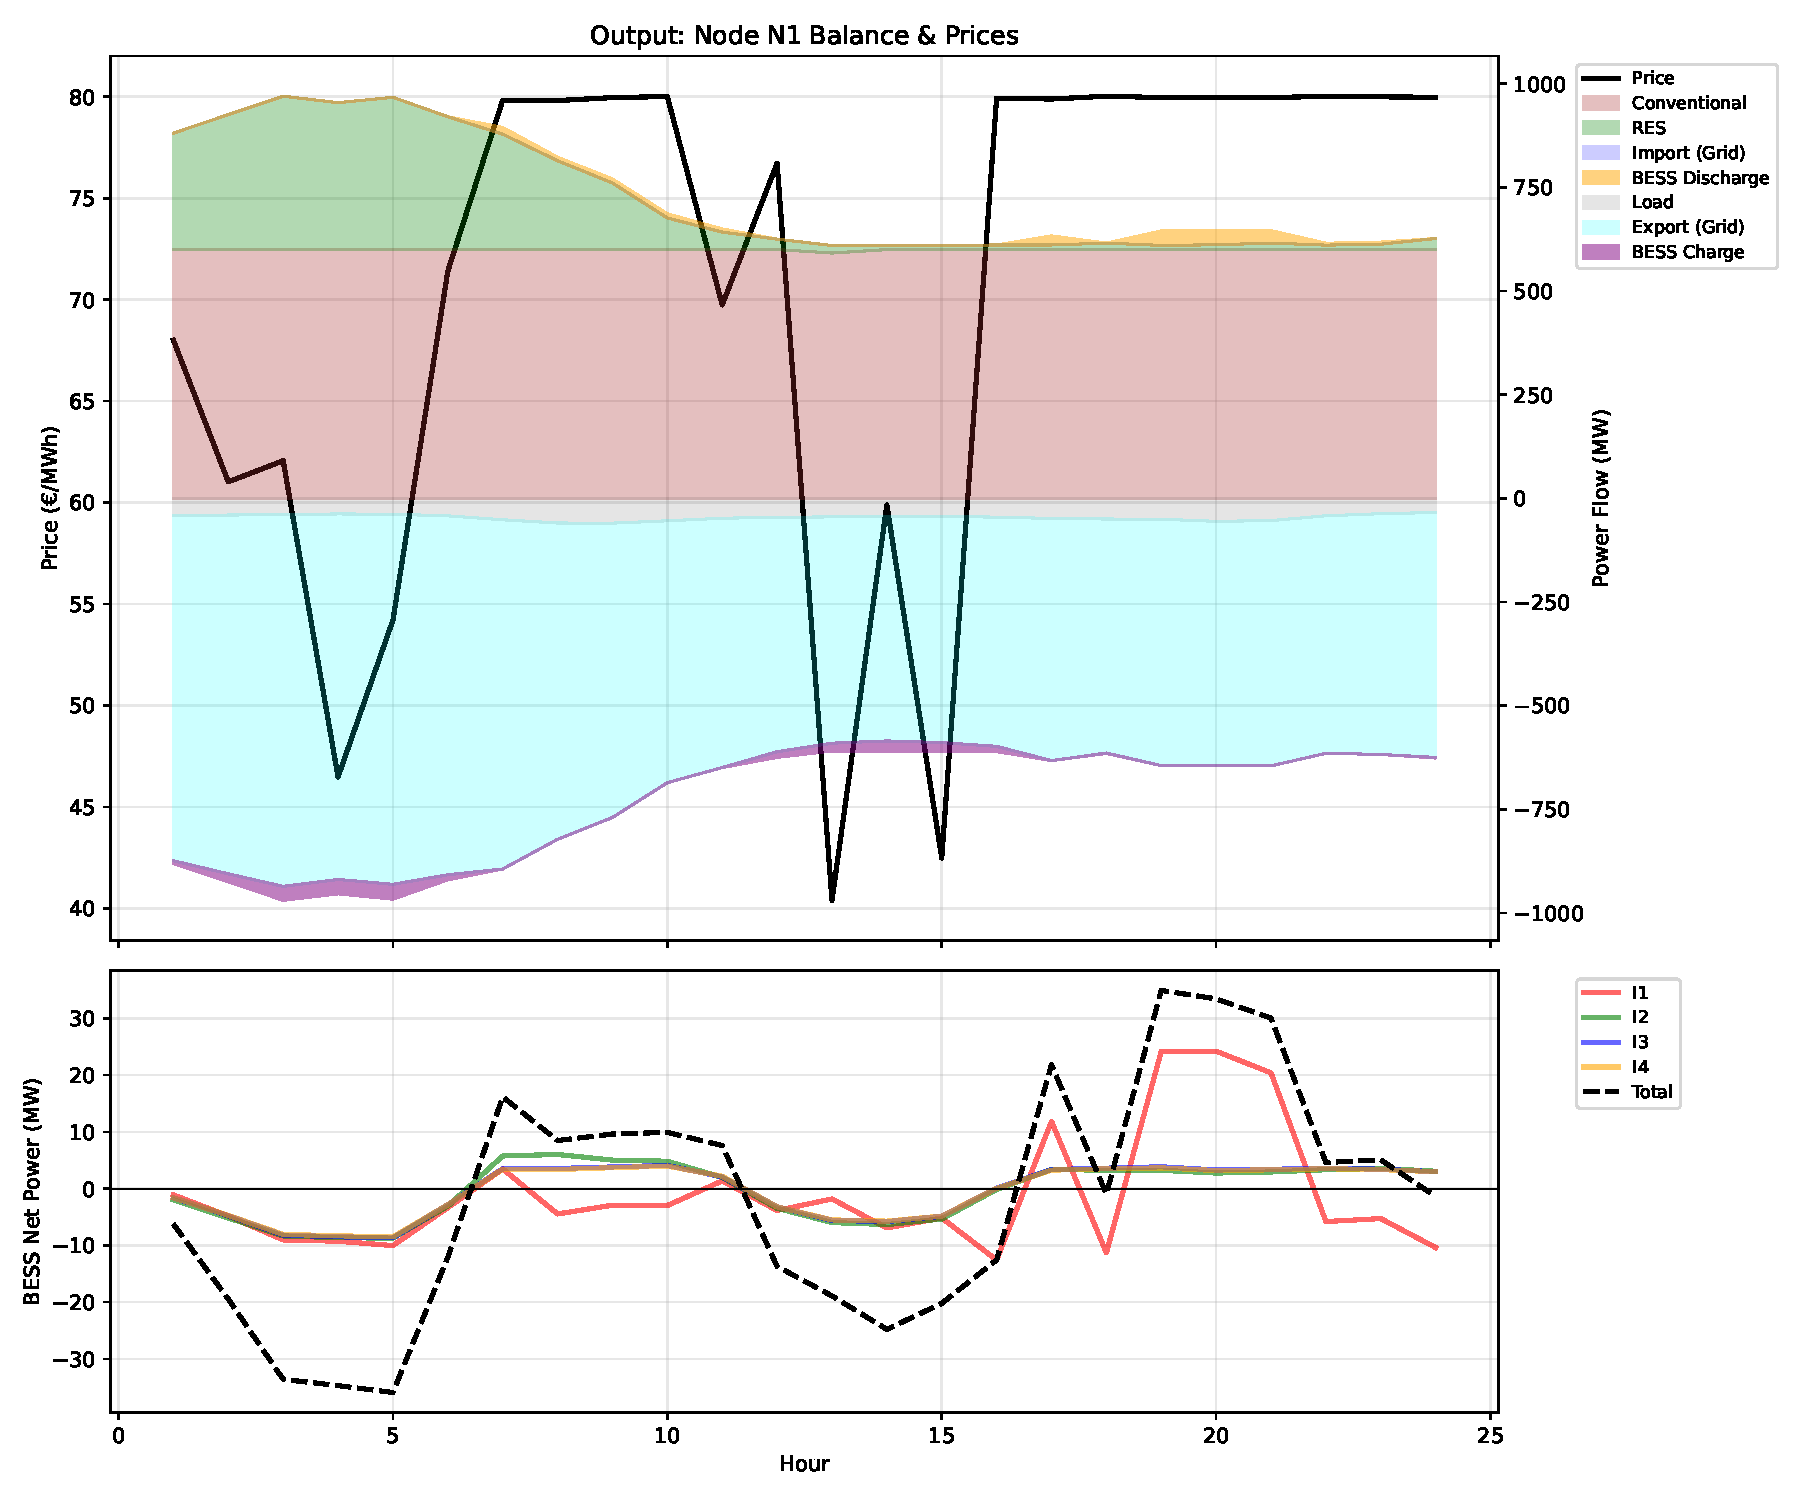
\includegraphics[width=\linewidth]{figures/with_aFRR_N1_Balance.pdf}
        \caption{Node 1 (Multi-Service)}
        \label{fig:n1_multi}
    \end{subfigure}
    \hfill
    \begin{subfigure}{0.75\linewidth}
        \centering
        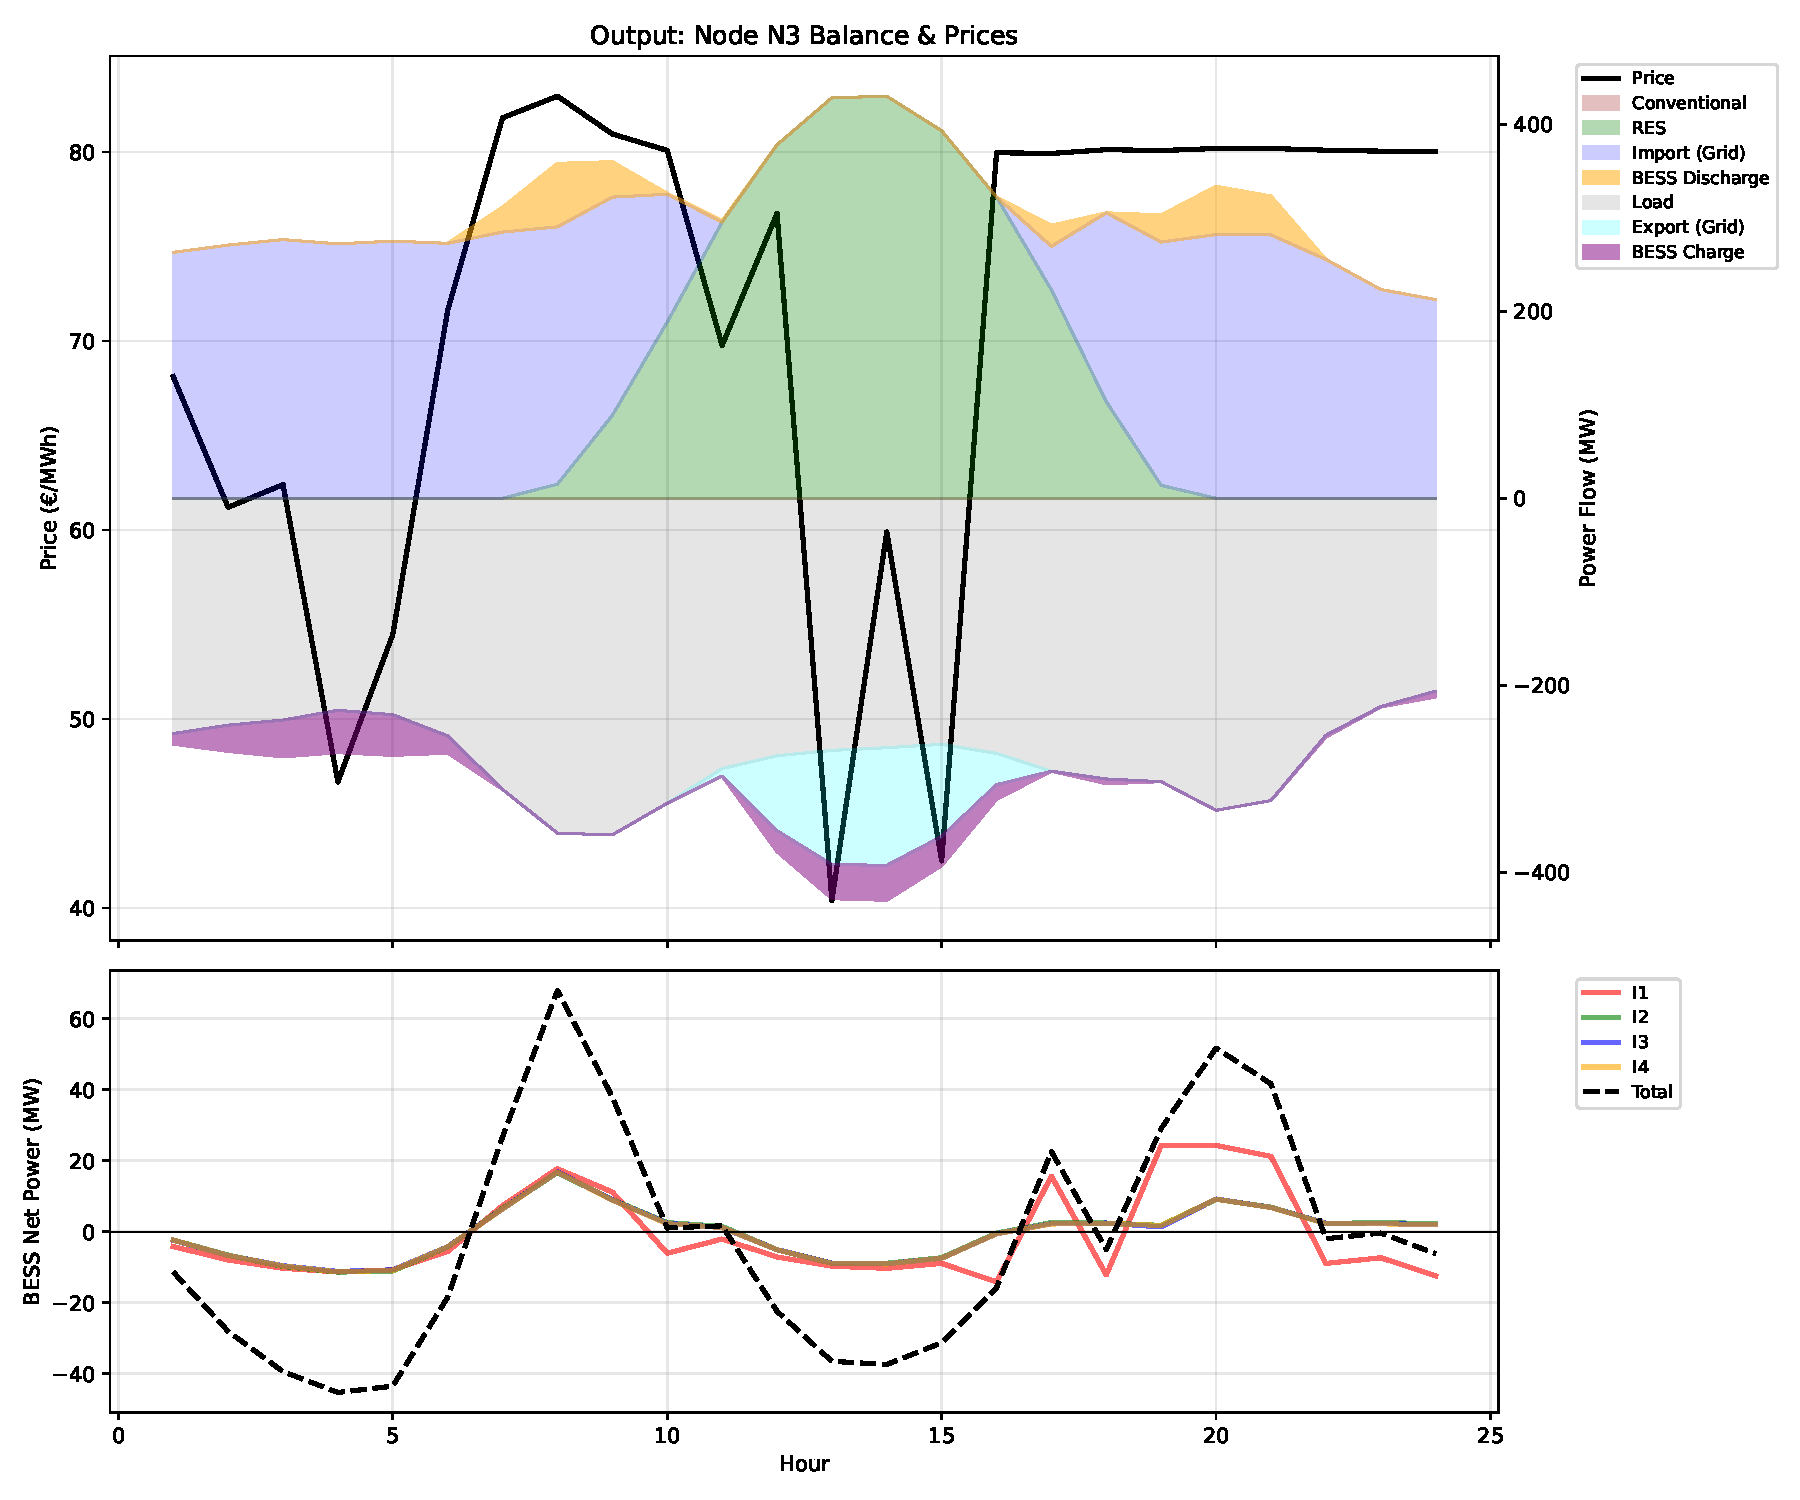
\includegraphics[width=\linewidth]{figures/with_aFRR_N3_Balance.pdf}
        \caption{Node 3 (Multi-Service)}
        \label{fig:n3_multi}
    \end{subfigure}
    \caption{Nodal balances in the Multi-Service Scenario. The aFRR obligations synchronize BESS operations and price dynamics across structurally different nodes.}
    \label{fig:n3_balance}
\end{figure}